\documentclass{scrartcl}
\usepackage[a4paper,left=1in,right=1in,top=1.2in,bottom=1in]{geometry}
\usepackage{siunitx}
\usepackage{graphicx}
\setkomafont{disposition}{\normalfont\bfseries}

%title
\title{Exercise 01:\\Linear recurrent network}
\subtitle{Theoretical Neuroscience II}
\author{Johannes G\"atjen \and Lorena Morton}

%use these for structure/overview
\newcommand\Question{%
  \textbf{Question:}%
}
\newcommand\Answer{%
  \textbf{Answer:}%
}

\begin{document}
\maketitle
%include picture
\begin{figure}[h]
\centering
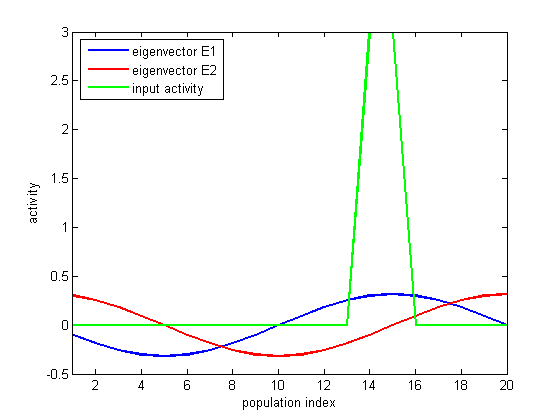
\includegraphics[trim = {0.6cm 0 1.2cm 0.7cm}, width=0.7\textwidth, clip]{../pics/eigen}
\caption{Visualization of network connectivity eigenvectors (red and blue) and an example input (green), as a function of population index.}
\label{label}
\end{figure}

\begin{figure}[h]
\centering
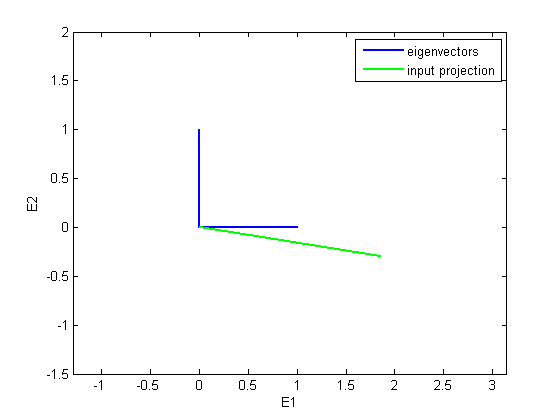
\includegraphics[trim = {0.6cm 0 1.2cm 0.7cm}, width=0.7\textwidth, clip]{../pics/input}
\caption{An example input (green) projected onto the plane of the two principal eigenvectors, shown in blue.}
\label{label}
\end{figure}

The steady state solutions are weighted sums of the eigenvectors. The weights depend on the similarity of the input to the eigenvector, as well as the eigenvalue. The closer the eigenvalue is to one, the higher the resulting amplitude of the steady state.

\begin{figure}[h]
\centering
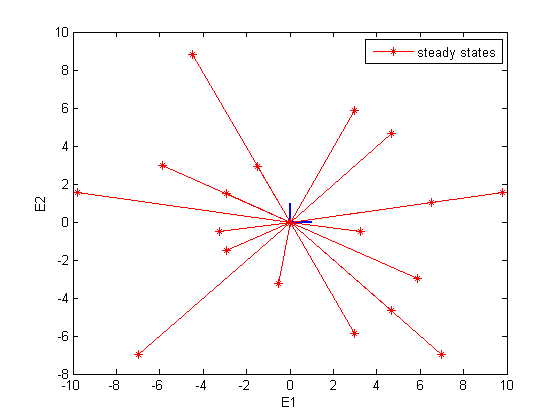
\includegraphics[trim = {0.6cm 0 1.2cm 0.7cm}, width=0.7\textwidth, clip]{../pics/steady}
\caption{The steady states (red asterisks) corresponding to several different inputs, projected on the eigenvector plane.}
\label{label}
\end{figure}

\begin{figure}[h]
\centering
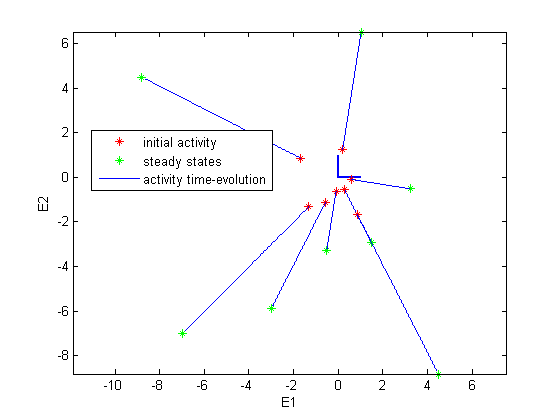
\includegraphics[trim = {0.6cm 0 1.2cm 0.7cm}, width=0.7\textwidth, clip]{../pics/time_evo}
\caption{The time evolution of the network for several different inputs, projected on the eigenvector plane. The input (=initial activity) is indicated by red asterisks. Over time the population activity moves towards the steady states, indicated by green asterisks.}
\label{label}
\end{figure}

\begin{figure}[h]
\centering
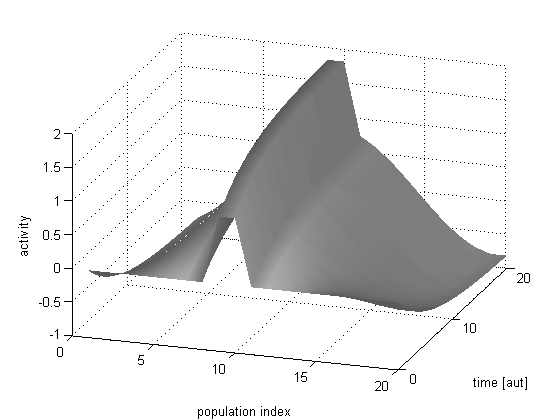
\includegraphics[trim = {0.4cm 0 0.7cm 0.7cm}, width=0.7\textwidth, clip]{../pics/all}
\caption{Visualization of the time evolution of the network activity for one example input.}
\label{label}
\end{figure}
%include picture
%\begin{figure}
%\centering
%\includegraphics[trim = {1.3cm 0 2cm 0.9cm}, width=\textwidth, clip]{../pics/picname}
%\caption{caption text}
%\label{label}
%\end{figure}
\end{document}